\subsection{Spezielle Relativitätstheorie}
\subsubsection{Koordinatentransformation und Newtonsche Mechanik}
Newtonsches Gesetz für N- Teilchen ist
\begin{eqnarray*}
m_i\ddot{\vec r}_i(t) = \vec F_i = - \frac{\partial V}{\partial \vec r_i}\\
\text{ mit }V(\vec r_1 , \dots, \vec r_N) = \sum \limits_{i<j} V_{ij}(\left|\vec r_i-\vec r_j\ri|)
\end{eqnarray*}
Wir betrachten die Koordinatentransformationen der Form
\begin{eqnarray*}\label{eq1}
\vec r' = \underbrace{\overleftrightarrow D \vec r}_{\text{Drehung}} + \underbrace{\vec vt}_{\text{gleichförmige Bewegung}} + \underbrace{\vec a}_{\text{Translation}}
\end{eqnarray*}
Für die Drehmatrix muss gelten $\overleftrightarrow D^{-1} = \overleftrightarrow D^T$. Die Geschwindigkeit $\vec{v}$ ist bei einer Galileotransformation konstant.\\ \\


Koordinatensysteme, die durch Galileotransformationen verbunden sind, heißen {\bf Inertialsysteme}(IS).\\

Zu zeigen ist: Das Newtonsche Gesetz ist unter den obigen Transformationen forminvariant.\\
Einziger nicht trivialer Fall ist die Drehtransformation, bei der gilt
\begin{eqnarray*}
\ddot{\vec r}_i' = \overleftrightarrow D\ddot{\vec r}_i \qquad \qquad
\left|\vec r'_i-\vec r'_j\ri|^2 \g \Big(\overleftrightarrow D(\vec
  r_i-\vec r_j)\Big)^T \Big (\overleftrightarrow D(\vec r_i-\vec
  r_j)\Big)\\ 
(\vec r_i-\vec r_j)^T \ \overleftrightarrow D^T \g (\vec r_i-\vec
r_j)^T \ \overleftrightarrow D^{-1} \longrightarrow \left|\vec
  r'_i-\vec r'_j \ri|^2 = \left|\vec r_j-\vec r_i\ri|^2\\ 
\end{eqnarray*}
\begin{eqnarray*}
\vec F'_i = -\frac {\partial}{\partial \vec r_i'}V = -
\overleftrightarrow D\frac{\partial V}{\partial \vec r_i} =
\overleftrightarrow D\vec F_i\\ 
m_i\ddot{\vec r}_i' = m_i \overleftrightarrow D\ddot{\vec r}_i =
\overleftrightarrow D \vec F_i = \vec F_i' 
\end{eqnarray*}
$\Longrightarrow$ Das Newtonsche Gesetz ist forminvariant.
\\
\\

Bemerkung:
\begin{itemize}
\item Äquivalente Formulierung:\\
Die Abstände zweier Punkte sind in allen Inertialsystemen gleich (d.h. $\Delta r = \left|\vec r_1 -\vec r_2\ri|=\left|\vec r_1' -\vec r_2'\ri|=\Delta r'$).
\item Relativitätsprinzip:\\
In allen Inertialsystemen sind die physikalischen Gesetze gleich.
\end{itemize}


\subsubsection{Elektrodynamik}
Wellengleichung im Vakuum:
\begin{eqnarray*}
\left[\frac{\partial^2}{\partial \vec r^2} - \frac 1 {c^2} \frac {\partial^2}{\partial t^2}\right] \vec E = 0
\end{eqnarray*}
Die Wellengleichung ist forminvariant unter Drehung und Translation, wie besipielsweise $\vec{r}'=\overleftrightarrow D\vec{r}+\vec{a}$ oder $E'(\vec{r},t)=\overleftrightarrow D E(\vec{r},t)$.
Eine mögliche Lösung ist: Kugelwelle, definiert durch eine Wellenfront
\begin{eqnarray*}
\vec r^2 - c^2t^2 = const.  = 0
\end{eqnarray*}
Was passiert unter $\vec r' = \vec r + \vec v t$ ?
\begin{eqnarray*}
(\vec r'+ \vec v t)^2 - c^2 t^2 = const.
\end{eqnarray*}

\begin{wrapfigure}{l}{5cm}
\begin{center}
	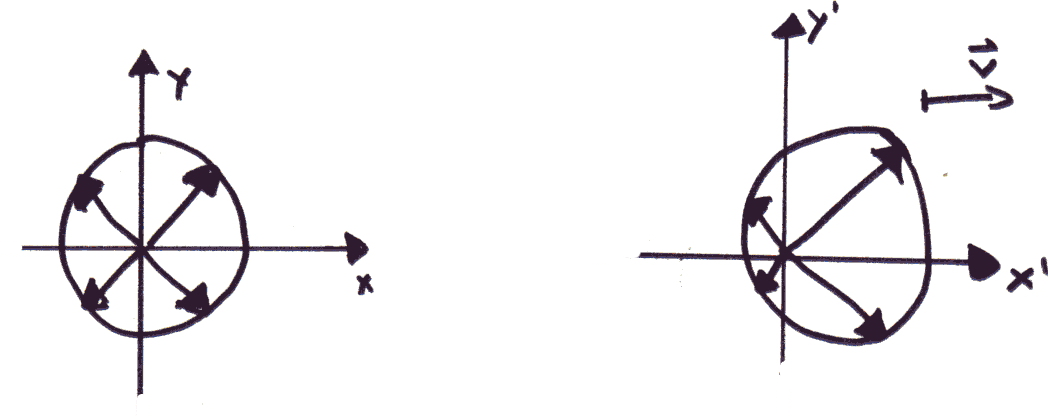
\includegraphics[scale=0.10]{Figs/Pim00013.png}
\end{center}
\end{wrapfigure}

$\longrightarrow$ Die Ausbreitungsgeschwindigkeit hängt von der Richtung ab! Dies steht im Widerspruch zu der aus den Maxwellgleichungen gefolgerten Wellengleichung. Eine der beiden Theorien muss also falsch sein. 

Dies ist im Widerspruch zum Experiment von Michelson und Morley (1887), welches zeigt, dass die Lichtgeschwindigkeit in \underline{allen} Inertialsystemen gleich ist.\\ \\
\underline{Lösung:} Einstein (1905) postuliert, dass die Lichtgeschwindigkeit in allen Inertialsystemen gleich ist.\\ \\
Konsequenzen:
\begin{itemize}
\item Die Galilei-Transformationen sind nicht mehr die korrekte Koordinatentransformation.
\item Die Newtonsche Mechanik ist nicht mehr gültig.
\item Die Zeitmessung hängt vom Inertialsystem ab. Die Zeit ist nicht mehr absolut.
\end{itemize}\vspace{1.5cm}
Beispielsweise sind die Maxwell-Gleichungen nicht invariant unter der Galilei-Transformationen.\\
\\
$\longrightarrow$ Einstein ersetzt die Galilei-Transformation durch die Lorentztransformation.\\

\subsubsection{Lorentztransformationen}
Gesucht ist die Transformation, die einen Lichtkegel invariant lässt:
\begin{eqnarray*}
\vec {r'}^2 - c^2 {t'}^2 = \vec r ^ 2 - c^2t^2
\end{eqnarray*}
Wir wählen den Ansatz einer linearen Transformation ($\vec r, t \rightarrow \vec r ',t'$) zwischen Inertialsystemem, die sich in x-Richtung mit einer Geschwindigkeit $\vec v$ gegeneinander bewegen.
\begin{alignat*}{5}
\text{Annahme:}\qquad \qquad &y' = y \qquad  \qquad \qquad \qquad \qquad  &z' \g z&\\
&t' = \gamma t- \gamma\beta \frac x c\qquad  &x' \g \gamma &x - \gamma\beta t \cdot c
\end{alignat*}
Der Ursprung sei bei $x' = 0$
\begin{eqnarray*}
\longrightarrow x = \beta c t  = v t \Rightarrow \boxed{\beta = \frac v c}\\
{\vec r}^{'2} -c^2{t}^{'2} = \vec r^2- c^2t^2 \Rightarrow \dots \Rightarrow\\
\boxed{\gamma = \frac1 {\sqrt{1 - \frac{v^2}{c^2}}} = \frac 1 {\sqrt{1- \beta^2}}}
\end{eqnarray*}
Dies sind die Lorentztransformationen (,,Boosts''):
\begin{eqnarray*}\boxed{
x' = \frac x  {\sqrt{1 - \frac{v^2}{c^2}}} - \frac{v t}{\sqrt{1 - \frac {v^2}{c^2}}}}\\\boxed{
t' = \frac t {\sqrt{1 - \frac{v^2}{c^2}}} - \frac{v \frac x{c^2}}{\sqrt{1 - \frac{v^2}{c^2}}}}
\end{eqnarray*}
Im Grenzfall $v\ll c$ wird aus den Lorentztransformationen die Galileitransformation und aus $t'$ wird $t$.

\vspace{1.5cm}
\underline{Transformationen im Minkowskidiagramm}\\
Die  Rücktransformation ist gegeben durch:
\begin{eqnarray*}
x = \gamma x' + \gamma \beta c t'\\
t = \gamma t' + \gamma \frac{\beta}  c x'
\end{eqnarray*}
Dies hat folgende physikalische Folgen:\\
\begin{wrapfigure}{l}{5.5cm}
\begin{center}
	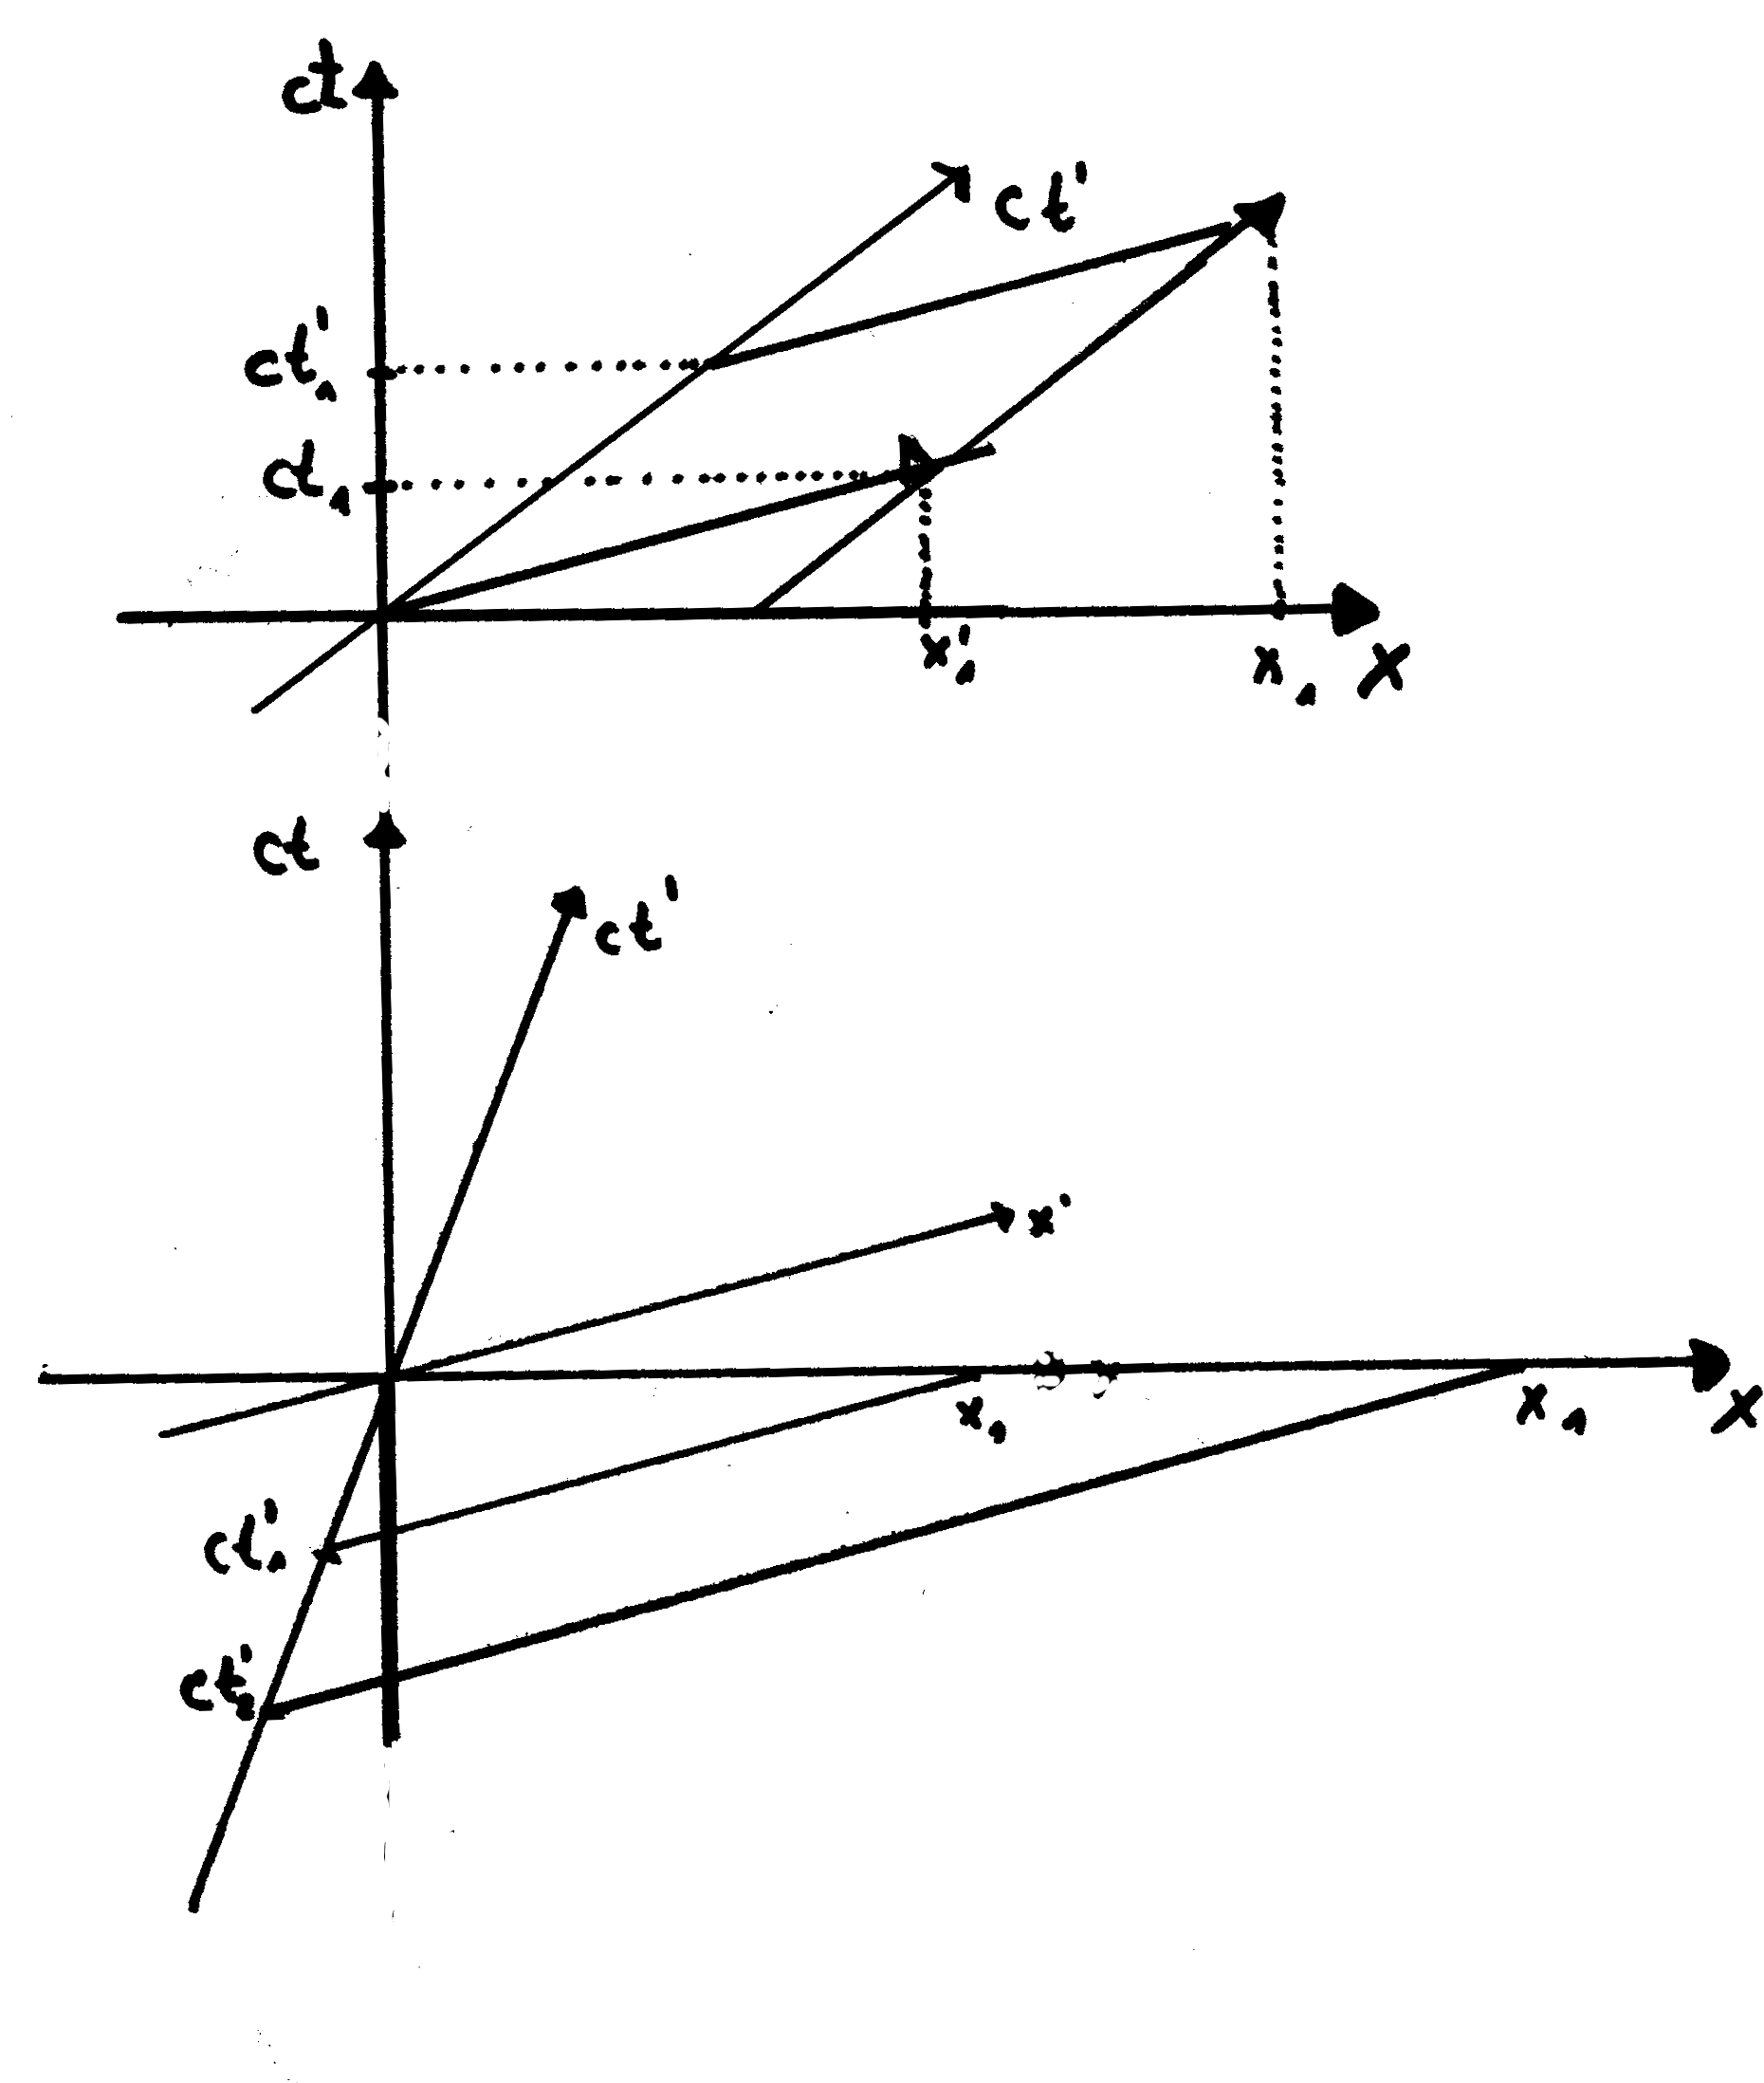
\includegraphics[scale=0.10]{Figs/Pim00012.png}
\caption{Minkowskidiagramm, unten: Relativität der Gleichzeitigkeit}
\end{center}
\end{wrapfigure}

\begin{itemize}


\item {Relativität der Gleichzeitigkeit:}\\
Zwei Ereignisse an verschiedenen Orten $x_1$ und $x_2$ zur Zeit $t=0$ im IS  sind nicht gleichzeitig im IS '.
\begin{eqnarray*}
t'_2-t'_1 \g -\beta \gamma \cdot \frac{(x_2-x_1)} c \neq 0\\
x'_2-x'_1 \g \gamma(x_2-x_1)\\
\Rightarrow (t'_2-t'_1) \g \frac {-\beta}c (x'_2-x'_1)
\end{eqnarray*}

\item {Zeitdilatation:}\\
Bei $x=0$ ist im IS' die Zeitdifferenz größer als im IS.
\begin{eqnarray*}
t'_2-t'_1 = \gamma(t_2-t_1) \ge t_2-t_1
\end{eqnarray*}

\item{Längenkontraktion:}\\
Der Wegunterschied $x_2-x_1$ ist zur Zeit $t'_2 = t'_1$  im IS'  geringer als im IS, d.h.\\ $x'_2-x'_1< x_2-x_1$.\\
\\




\begin{eqnarray*}
x'_2-x'_1 \g \gamma (x_2-x_1) - \beta\gamma(t_2-t_1) c\\
t'_2 - t'_1 = 0 \g \gamma (t_2-t_1) - \beta \gamma (x_2-x_1)\frac 1 c\\
\longrightarrow t_2-t_1 \g \beta \frac{(x_2-x_1) } c\\
\Longrightarrow x'_2 -x'_1 \g \gamma(1-\beta^ 2)(x_2-x_1) = \frac{(x_2-x_1)} {\gamma}
\end{eqnarray*}


\end{itemize}
\begin{center}
	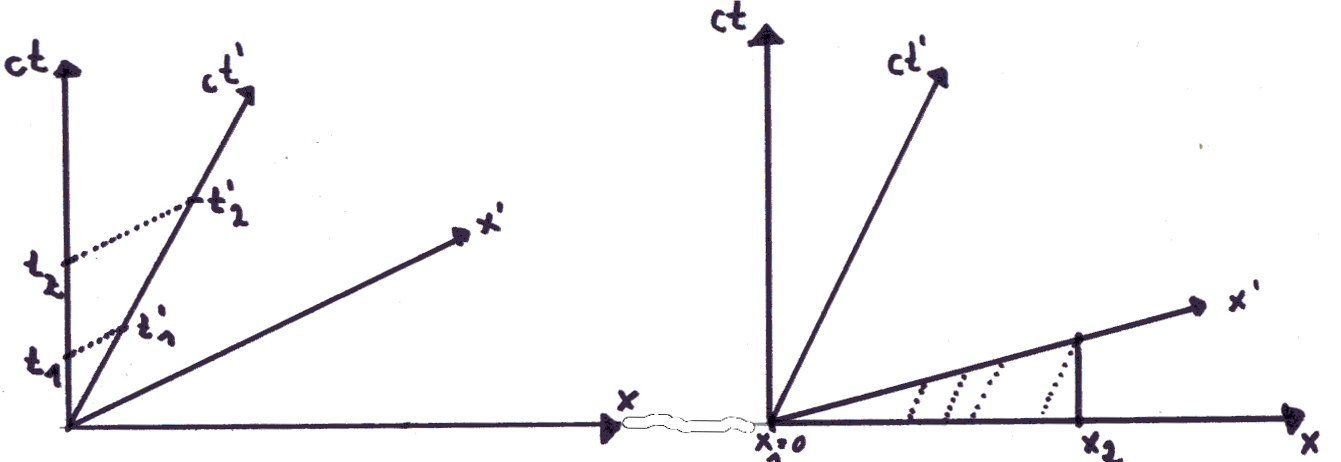
\includegraphics[scale=0.20]{Figs/Pim000111.png}
	\captionof{figure}{links: Zeitdilatation; rechts : Längenkontraktion}
\end{center}

\begin{itemize}
\item{ Kausalität bezüglich einem dem Ereignis im Ursprung}\\
Maximale Verschiebung liegt bei $ct = |\vec r| \ \ \ \rightarrow$ 45 \grat Verschiebung\\
$\Longrightarrow$ Lichtkegeloberfläche ist bei $|\vec r| = ct$\\
Ereignisse mit $|\vec r|^ 2<c^2 t^ 2$ befinden sich im Lichtkegel.\\
\begin{itemize}
\item Ereignisse mit $|\vec r|^ 2<c^2 t^ 2$ heißen {\bf zeitartig} und können mit $v<c$ erreicht werden.
\item Ereignisse mit $|\vec r|^ 2 > c^ 2t^ 2$ heißen {\bf raumartig} und können nicht erreicht werden.
\item Ereignisse mit $|\vec r| ^ 2 = c^2t^ 2$ heißen {\bf lichtartig} und können mit $v=c$ erreicht werden.

\begin{center}
	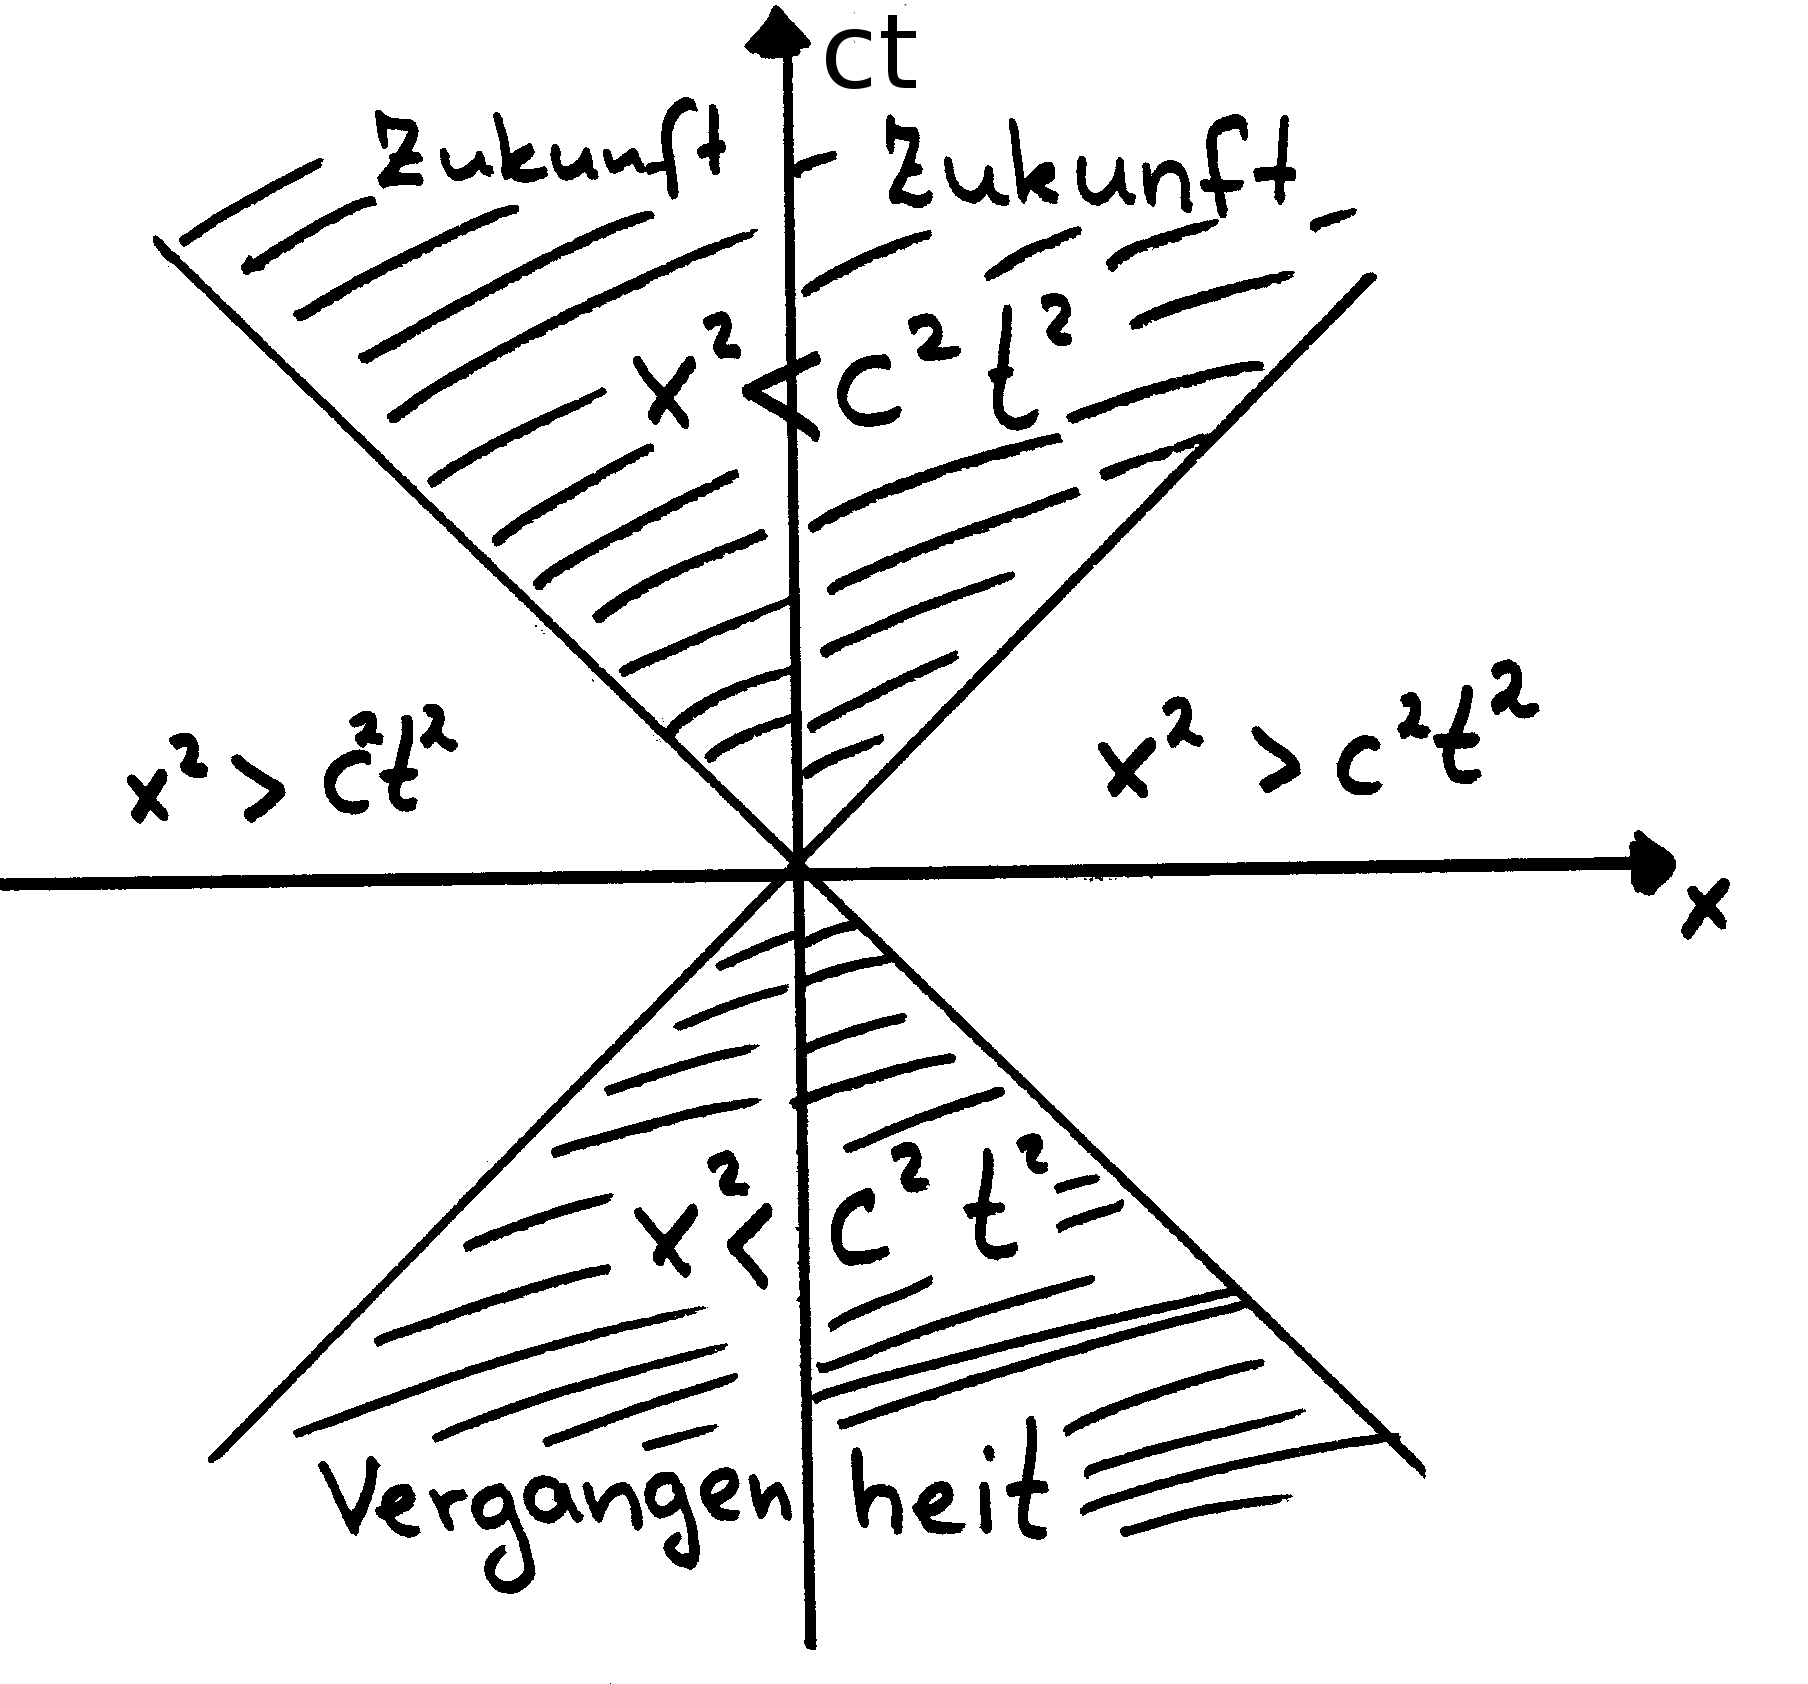
\includegraphics[scale=0.10]{Figs/Pim000112.png}
	\captionof{figure}{links: Zeitdilatation; rechts : Längenkontraktion}
\end{center}

\end{itemize}
Für Lorentztransformationen gilt: 
\begin{eqnarray*}
|\vec r|'^ 2-c^ 2t'^ 2 = |\vec r|^ 2- c^ 2t^ 2
\end{eqnarray*}
$\Longrightarrow$ Die Kausalität bleibt erhalten.
\end{itemize}

\subsubsection{Vierervektoren / Tensorrechnung}
Wir fassen Zeit und Raum zu einem sog. Vierervektor zusammen:
\begin{eqnarray*}
x \g (ct,x,y,z) = (x_0,x_1,x_2,x_3)\\
x^{\mu} \g \left ( \begin{array}{c} ct\\ x\\y\\z\end{array} \ri) = \left ( \begin{array}{c} ct\\ \vec r \end{array}\ri )
\end{eqnarray*}
Mit den Konventionen:
\begin{eqnarray*}
x^ 0 = c\cdot t \qquad x^ 1 = x \qquad x^ 2 = y \qquad x^ 2 = z
\end{eqnarray*}
\begin{center}
\begin{tabular}{cccccc}
\end{tabular}\end{center}
Lorentztransformationen lassen die Größe $c^ 2t^ 2 - \vec r^ 2$ invariant.\\
Definiere entsprechendes Skalarprodukt:
\begin{eqnarray*}
x^ 2_{\nu} = \sum \limits_{\mu = 0}^ 3 x^ {\mu} g_{\mu \nu} x^ {\nu} = c^ 2t^ 2- \vec r^ 2
\end{eqnarray*}
mit dem metrischen Tensor (Metrik):
\begin{eqnarray*}
g_{\mu\nu} = \left ( \begin{array}{cccc} +1&0&0&0\\0&-1&0&0\\0&0&-1&0\\0&0&0&-1\end{array} \ri)\\
g_{00} = 1 \qquad g_{ii} = -1 \qquad g_{\mu\nu} = 0 \text{ für  } \mu \neq \nu
\end{eqnarray*}
Definiere den kovarianten Vektor:
\begin{equation*}
 x_{\nu}=\sum_{\mu}g_{\mu\nu}x^{\mu}=(ct,-x,-y,-z)\quad\Rightarrow\quad x^2=\sum_{\nu}x_{\nu}x^{\nu}
\end{equation*}

\underline{Einsteinsche Summenkonvention}
Über wiederholt auftretende Indizes wird summiert.\\
Meist ist ein Index oben und einer unten gesetzt.\\
Lorentztransformation:
\begin{eqnarray*}
x'{}^{\mu} \g \Lambda^{\mu}_{\ \ \nu} \ \ x^{\nu}\\
\text{mit z.B. } \Lambda_{\ \ \nu}^{\mu} \g \left ( \begin{array}{cccc} \gamma&-\beta\gamma&0&0\\ -\beta \gamma&\gamma&0&0\\ 0&0&1&0\\0&0&0&1 \end{array} \ri)=\frac{\partial x'^{\mu}}{\partial x^{\nu}}
\end{eqnarray*}
Das Skalarprodukt ist invariant unter einer Lorentztransformation.
\begin{eqnarray*}
{x'}^2 \g {x'} ^{\mu} g_{\mu\nu} {x'}^{\nu} = x^{\lambda}\ \Lambda _{\ \ \lambda}^{\mu}\  \ g_{\mu\nu} \  \Lambda_{\ \ \kappa}^{\nu}\ \ x^{\kappa} \\ \g x^{\lambda} g_{\lambda \kappa} x^{\kappa}
\end{eqnarray*}
$\Longrightarrow$ Die Metrik ist in beiden Inertialsystemen die gleiche. (Dies folgt aus der Form der Lorentztransformation.)
\begin{itemize}
\item Es gilt ebenfalls:
\begin{eqnarray*} x \cdot y \g x^{\mu} \ g_{\mu\nu} \ y^{\nu} \\ \g x_0y_0 - x_1y_1-x_2y_2-x_3y_3 \end{eqnarray*}
\item Abstandsquadrat  $ds^2$\\
\begin{eqnarray*} ds^2 = dx^{\mu} \ g_{\mu \nu} dx^{\nu} = c^2dt^2 - d\vec r^2\end{eqnarray*}
Hieraus folgt, dass das Abstandsquadrat größer null, gleich null und kleiner null sein kann.\\
$\longrightarrow$ ,,pseudoeuklidischer Raum''
\end{itemize}
\vspace{1.5cm}
\underline{Verallgemeinerung der Vektoren auf {\bf Tensoren}.}
\begin{itemize}
\item {\bf Skalare (Tensoren 0. Stufe) }\\  Skalare ändern sich nicht unter einer Lorentztransformation ($s'(x') = s(x)$).\\
(Zum Beispiel : Skalarprodukt, Lichtgeschwindigkeit $c$, Ruhemasse,...)
\item {\bf Vektoren (Tensoren 1. Stufe)} Vektoren werden mit der Lorentztransformation transformiert.\\
Unterscheide zwischen:
\begin{itemize}
\item {\bf Kontravariante Vektoren}\\
\begin{eqnarray*} {A'}^{\mu} = \Lambda_{\ \ \nu}^{\mu} \ \ A^{\nu} \qquad \qquad
\big ( {x'}^{\mu} = \underbrace{\frac{\partial {x'}^{\mu}}{\partial x^\nu}}_{\Lambda_{\ \ \nu}^{\mu}} x^{\nu} \big)
\end{eqnarray*}
\item{\bf Kovariante Vektoren}\\ \begin{eqnarray*} B'_{\mu} = \Lambda_{\ \ \mu}^{\nu}\ \ B_{\nu} \qquad \qquad \big ( x'_{\mu} = \underbrace{\frac{\partial x^{\nu}}{\partial {x'}^{\mu}}}_{\Lambda_{\ \ \mu}^{\nu}}x_{\nu} \big )\end{eqnarray*}
\end{itemize}
Diese Vektoren können mit dem metrischen Tensor ineinander umgerechnet werden:
\begin{eqnarray*} B^{\mu} = g^{\mu\nu} B_{\nu}\end{eqnarray*}
Für das Skalarprodukt ergibt sich:
\begin{eqnarray*} AB = A^{\mu}B_{\mu} = A^{\mu} g_{\mu\nu} B^{\nu} \end{eqnarray*}
Als Beispiel kann der Vierervektor $x$ betrachtet werden:
\begin{eqnarray*}
x^{\mu} \g \Big ( ct, x,y,z \Big)\\ x_{\mu} \g g_{\mu\nu} B^{\nu} = \Big ( ct, -x,-y,-z\Big)
\end{eqnarray*}
Jedoch gilt für die Ableitungen:
\begin{alignat*}{6} \frac{\partial}{\partial x^{\mu}} \g \Big(\frac{\partial}{\partial ct}\ ,\frac{\partial}{\partial x} \ ,\frac{\partial}{\partial y}\ ,\frac{\partial}{\partial z} \Big ) \g \partial_{\mu} \qquad&\rightarrow& \quad \text{Kovariant}\\
\frac{\partial}{\partial x_{\mu}} \g \Big ( \frac{\partial}{\partial ct}\ ,\frac{-\partial}{\partial x}\ , \frac{-\partial}{\partial y}\ ,\frac{-\partial}{\partial z}\Big ) \g \partial^{\mu} \quad &\rightarrow& \quad \text{Kontravariant}
\end{alignat*}
Die obigen Gleichungen folgen aus der Umformung
\begin{eqnarray*} \frac{\partial}{\partial{x'}^{\mu}} = \underbrace{\frac{\partial x^{\nu}}{\partial{x'}^{\mu}}}_{\Lambda_{\ \ \mu}^{\nu}} \frac{\partial}{\partial x^{\nu}} \end{eqnarray*}
Die Divergenz ist wiederum ein Skalar $\partial_{\mu} A^{\mu} = \frac{\partial A^0}{\partial ct} + \nabla \vec A$

\item{\bf Tensoren höherer Stufe}\\
Tensoren der Stufe $k$ sind über ihr Transformationsverhalten unter $k$ Lorentztransformationen definiert.
\begin{eqnarray*}
{T'}^{\mu_1 \mu_2 \dots \mu_k} = \Lambda_{\ \ \nu_1}^{\mu_1} \ \ \Lambda_{\ \ \nu_2}^{\mu_2} \cdots \Lambda_{\ \ \nu_k}^{\mu_k}\ \ T^{\nu_1\nu_2\dots \nu_k} \end{eqnarray*}
$\longrightarrow$ Kontravariante Tensoren der $k$-ten Stufe (kovariant analog).\\ 
Für gemischte Terme gilt:
\begin{eqnarray*}
{T'}_{\ \ \ \  \ \ \ \ \mu_1 \dots\mu_k}^{\lambda_1 \dots \lambda_p} = \Lambda_{\ \ \mu_1}^{\nu_1} \cdots \Lambda_{\ \ \mu_k}^{\nu_k}\ \  \Lambda_{\ \ \kappa_1}^{\lambda_1}\cdots \Lambda_{\ \ \kappa_p}^{\lambda_p} \ \ T_{\ \ \ \ \ \ \ \nu_1 \dots\nu_k}^{\kappa_1 \dots \kappa_p}
\end{eqnarray*}
\underline{Beispiele:} \begin{itemize}
\item \begin{eqnarray*} T_{\mu\nu} ^{\ \ \ \ \ \lambda\delta}= x_{\mu}A_{\nu}\ x^{\lambda} B^{\delta}\end{eqnarray*}
\item Verjüngung eines Tensors \begin{eqnarray*} T_{\ \ \ \ \ \ \ \ \ \ \ \ \mu_1 \dots \mu_k}^{\nu_1 \dots \nu_{p-1} \mu_k}\end{eqnarray*}
Dies ist ein Tensor (mit $k-1$ kontra- und $p-1$ kovariante).
\begin{eqnarray*} &\rightarrow& \qquad  \qquad T_{\mu}^{\mu} = g_{\mu\nu} T^{\mu\nu} \quad \text{skalar} \\
&\rightarrow& \qquad\qquad x_{\mu}y^{\mu} = g_{\mu\nu}x^{\mu}y^{\nu} \end{eqnarray*}
\end{itemize}
\item{\bf D'Alembertoperator}
\begin{eqnarray*} 
\Box = \partial_{\mu} \partial^{\mu} = \frac 1 {c^2} \frac {\partial^2}{\partial t} - \frac{\partial ^2}{\partial \vec r^2} \ \widehat = \text{ skalare Größe}
\end{eqnarray*}
\item{\bf Invarianz vom Skalarprodukt}
\begin{eqnarray*} A'_{\mu} {B'}^{\mu} = \underbrace{\frac {\partial x^{\nu}}{\partial{x'}^{\mu}}\frac{\partial {x'}^{\mu}}{\partial x^{\gamma}}}_{= \frac{\partial x^{\nu}}{\partial x^{\gamma}}} A_{\nu}B^{\gamma} = A_{\nu}B^{\nu} \quad \text{mit } \frac{\partial x^{\nu}}{\partial x^{\gamma}} = \delta_{\gamma}^{\nu} = \delta_{\nu,\gamma}
\end{eqnarray*}
\item \begin{eqnarray*} g_{\mu\nu}g^{\nu\kappa} = g_{\mu}^{\kappa} = \delta_{\mu}^{\kappa} = \underbrace{\delta{(\kappa \mu)}}_{\text{Kronecker-}\delta}\end{eqnarray*}
\end{itemize}
\subsubsection{Relativistische Mechanik}
Die Newtonsche Mechanik ist nicht Lorentzkovariant, da Ableitungen nach der Zeit in der Newtonschen Mechanik auftreten, welche nicht kovariant sind.
\begin{eqnarray*} \frac{dx^ {\mu}}{dt} = \big ( c, \dot{\vec r} \big)\end{eqnarray*}
Die Konstruktion einer relativistischen Mechanik wird mit Hilfe der sog. {\bf Eigenzeit $\tau$} entwickelt. Diese Eigenzeit ist gleich der Zeit, die in einem mitbewegten Koordinatensystem vergeht:
\begin{eqnarray*}
c^2d\tau^2 \g c^2{dt'}^2 -\underbrace{d\vec {r'}^2}_{= 0} = c^2{dt}^2 - d\vec r^2\\
\g c^2dt^2\Big ( 1- \frac{\vec v(t)^2}{c^2} \Big) \qquad \text{mit }\vec v = \frac{d\vec r}{dt}
\end{eqnarray*}
\begin{eqnarray*}
\rightarrow \boxed{d\tau = \frac 1 {\gamma(t)} dt} \end{eqnarray*}
Beachte: In obiger Gleichung ist $\gamma$ von der Geschwindigkeit des Teilchens abhängig!
\underline{Definitionen:} 
\begin{itemize} \item{\bf Vierergeschwindigkeit}\\
\begin{eqnarray*}
\frac{dx^{\mu}}{d\tau} \g u^{\mu} = \frac{d}{d\tau} \big( ct, \vec r\big ) = \gamma \frac d{dt} \big( ct, \vec r\big)\\ \g \gamma(c,\vec v) \end{eqnarray*}
Der Betrag dieser Vierergeschwindigkeit $u_{\mu}$ ist gegeben durch
\begin{eqnarray*} u_{\mu}u^{\mu} = \gamma^2c^2 - \gamma^2v^2 = c^2.\end{eqnarray*}
\item{\bf Viererimpuls}\begin{eqnarray*} p^{\mu} = m \ u^{\mu}\end{eqnarray*}
\end{itemize}
\underline{Modifiziertes Newtonsches Gesetz}
\begin{eqnarray*}
\frac d{d\tau} p^{\mu} = m \frac{du^{\mu}}{d\tau} =: K^{\mu}
\end{eqnarray*}
Bestimmung der sog. {\bf Minkowskikraft} $K^{\mu}$\\
Betrachte die drei Raumkomponenten:
\begin{eqnarray*} m \frac {du^i}{d\tau} = \frac{dp^i}{d\tau} = \gamma \frac{dp^i}{d t} = \gamma F^i = K^i \end{eqnarray*}
und die Zeitkomponente:
\begin{eqnarray*} 
\underbrace{  m  u_{\mu} \frac{d u_{\mu}}{d\tau}}_{ = \ u_{\mu} K^{\mu}\ = \ u_0K^0 - \gamma\vec v\vec K} \g \frac m 2 \frac{d}{d \tau} u_{\mu}u^{\mu} = \frac m 2 \frac{d}{d\tau} c^2 = 0\\
\Longrightarrow K^0 \g \underbrace{\frac 1 {\gamma c}}_{= \frac 1 {u_0}} \gamma \vec v\vec K = \gamma \frac{\vec v\vec F} c.
\end{eqnarray*}
Mit der Forderung der Invarianz der Lorentztransformation lässt sich die Minkowskikraft mit $K^0$ bestimmen.
\begin{eqnarray*} \Longrightarrow K^{\mu} = \gamma \Big( \frac{\vec v\vec F}c , \vec F\Big )\end{eqnarray*}
\underline{Betrag des Viererimpulses $ p_{\mu}p^{\mu} = m^2 c^2$}\\
\begin{eqnarray*} 
cp^0 \g m\gamma c^2 = \frac{mc^2}{\sqrt{1 - \frac {v^2}{c^2}}} \quad\text{Entwickle nach $v$ für }v\ll c\\
\g \underbrace{mc^2}_{E_{\text{ruhe}}} + \underbrace{\frac 1 2m v^2 }_{\text{nicht relat. }E_{\text{kin}} } + \frac 3 8 m \frac{v^4}{c^2} + \dots
\end{eqnarray*}
$\longrightarrow$ Identifiziere $cp^0$ mit der Energie $E$.\\
$\longrightarrow$ Relativistischer Energie-Impuls Zusammenhang:
\begin{eqnarray*} \boxed{ E = \sqrt{m^2c^4 + c^2\vec p^2}}\end{eqnarray*}
Für ein Teilchen in Ruhe reduziert sich die Gleichung auf
\begin{eqnarray*} \boxed{E = mc^2}\end{eqnarray*}
und zeigt die Äquivalenz von Masse und Energie.


%%% Local Variables: 
%%% mode: latex
%%% TeX-master: "main"
%%% End: 
